%Header und Footer Definitionen f�r das Deckblatt
\thispagestyle{fancy}
\renewcommand{\headrulewidth}{0mm}
\lhead{{\small }}
\chead{{\small }}
\rhead{{\small }}
\lfoot{{\small SIMPL � 2009 \$IMPL}}
\cfoot{{\small \docdate}}
\rfoot{{\small \thepage\ / \pageref{LastPage}}}


%Text f�r das Deckblatt
\vspace*{5cm}
\noindent{\LARGE Studienprojekt SIMPL} \\
\noindent\rule[1ex]{\textwidth}{1pt}
\vspace*{1cm}
\begin{flushleft}
	{\Huge \textbf{\doctitel}} \\
	\vspace{0.5cm}
	{\LARGE Version \docvers} \\
	\vspace{0.5cm}
	{\LARGE \docdate} \\
	\vspace{0.5cm}
	{\LARGE Verfasser: \docautor}
\end{flushleft}
\vspace*{1cm}
\noindent\rule[1ex]{\textwidth}{1pt}

\vspace*{2cm}
\begin{center}
	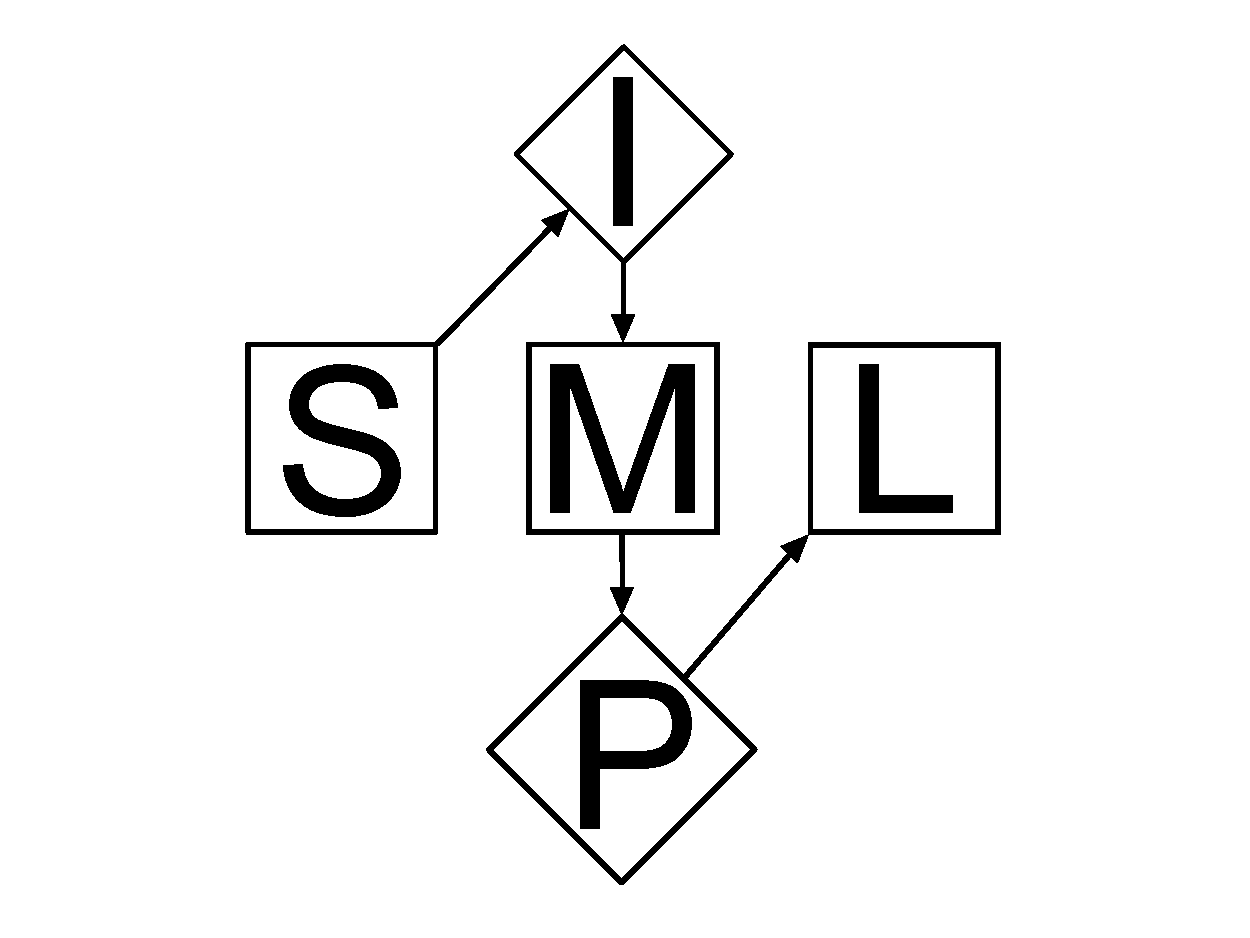
\includegraphics{SIMPL}
\end{center}

%Neue Seite beginnen
\pagebreak{}